\setlength{\columnsep}{3pt}
\begin{flushleft}
\bigskip
Step 4: MBR
\begin{itemize}
	\item BIOS checks for the \textbf{MBR} in the hard disk for the location of the \textbf{boot loader}.
	
	\item Let's see MBR in detail:
	\begin{figure}[h!]
		\centering
		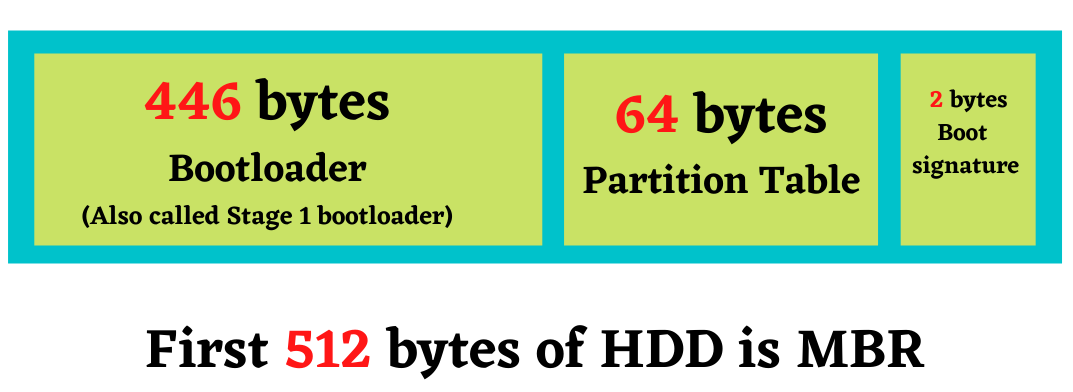
\includegraphics[scale=0.5]{content/chapter17/images/mbr.png}
		\caption{MBR}
		\label{fig:mbr}
	\end{figure}

	\begin{itemize}	
		\item MBR stands \textbf{Master boot recorder}.
		\item MBR is the first 512 bytes of hard drive.
		\item It contains:
		\begin{itemize}
			\item \textbf{Bootloader}: Also called \textbf{stage 1 bootloader}. It is of 446 bytes in size. More on this in next page.
			\item \textbf{Partition table}: Contains details about primary \& extended partition. Refer \textbf{Chapter 8: Partition under section 8.2.1} for more detail on this.
			\item \textbf{Boot signature also called magic number}: 
			\begin{itemize}
				\item Final 2 bytes are called the boot signature.
				\item Determine if the selected boot drive is bootable or not.
				\item On a disk that contains valid bootstrap code, the last two bytes will always be \textbf{0x55 0xAA}.
			\end{itemize}
			  
		\end{itemize}
	\end{itemize}
	
\end{itemize}

	
\end{flushleft}
\newpage


